
\section{Sparversion}
	Um Strom zu sparen, die Größe zu schrumpfen und Kosten günstiger zu werden, haben wir die \glqq Sparversion\grqq entwickelt.
	In dieser Variante der Gießanlage wurde die Anlage auf das wesentlichste beschränkt,das Gießen.
	Sie wurde so konzipiert, dass sie genau auf eine Pflanze zugeschnitten ist.
	Sie kann nur durch erneutes Programmieren auf andere Pflanzen und Böden angelernt werden. 	
	\subsection{Aufbau}
	In dieser Version wird auf das Display und die Kommunikation verzichtet.
	Dadurch wird viel der Verkabelung gespart, außerdem lässt sich die Hauptplatine deutlich kleiner gestalten.
	Der Wegfall zu weniger Platz"-bedarf des Systems führt und damit in ein kleineres Gehäuse passt.
	\subsection{Elektronik}
	Durch das wegfallen der XBee Platine und deren Beschaltung wird das 3,3\,V Netz nicht mehr benötigt.
	Dadurch reduziert sich die Größe der Hauptplatine auf \begin{math} 55 mm \times 32 mm \end{math}.
	Dies entspricht nicht nicht mal der Hälfte der Fläche der Version 1.1 mit \begin{math} 56 mm \times 65 mm \end{math}.
	\subsection{Programmierung}
	Um weiter Stromsparen zu können wurde diese Version nicht mit Arduino, sondern mit C geschriebenen Programm programmiert.
	Dies ermöglicht die Ausnutzung der Sleep Modi und die Interrupts des ATMega328. 
	Dadurch befindet sich der \glqq Arduino Nano\grqq \ hauptsächlich im Schlafmodus und verbraucht deutlich weniger Energie.
	Die Gießeinstellungen müssen auf Grund der fehlenden Kommunikation und Eingabemöglichkeiten über die Programmierung festgelegt werden.
	\subsubsection{Programmierwerkzeuge}
	Durch das Wegfallen der Arduino Bootloaders, kann die Hardware nicht mehr per USB programmiert werden. 
	Mit Hilfe des AVRISP mkII \footnote{\href{http://www.atmel.com/tools/avrispmkii.aspx}{www.atmel.com/tools/avrispmkii.aspx}} wird der Microcontroller direkt mit den Binärcode beschrieben. 
	Dazu wird der AVRISP mkII während des Betriebs des \glqq Arduino Nano\grqq\ an die ISP angesteckt. 
	Mit Hilfe der ISP-Schnittstelle lässt sich der Mikrocontroller direkt rogrammieren.
	\subsubsection{Logik}
		\begin{figure}[!h]
	\centering
	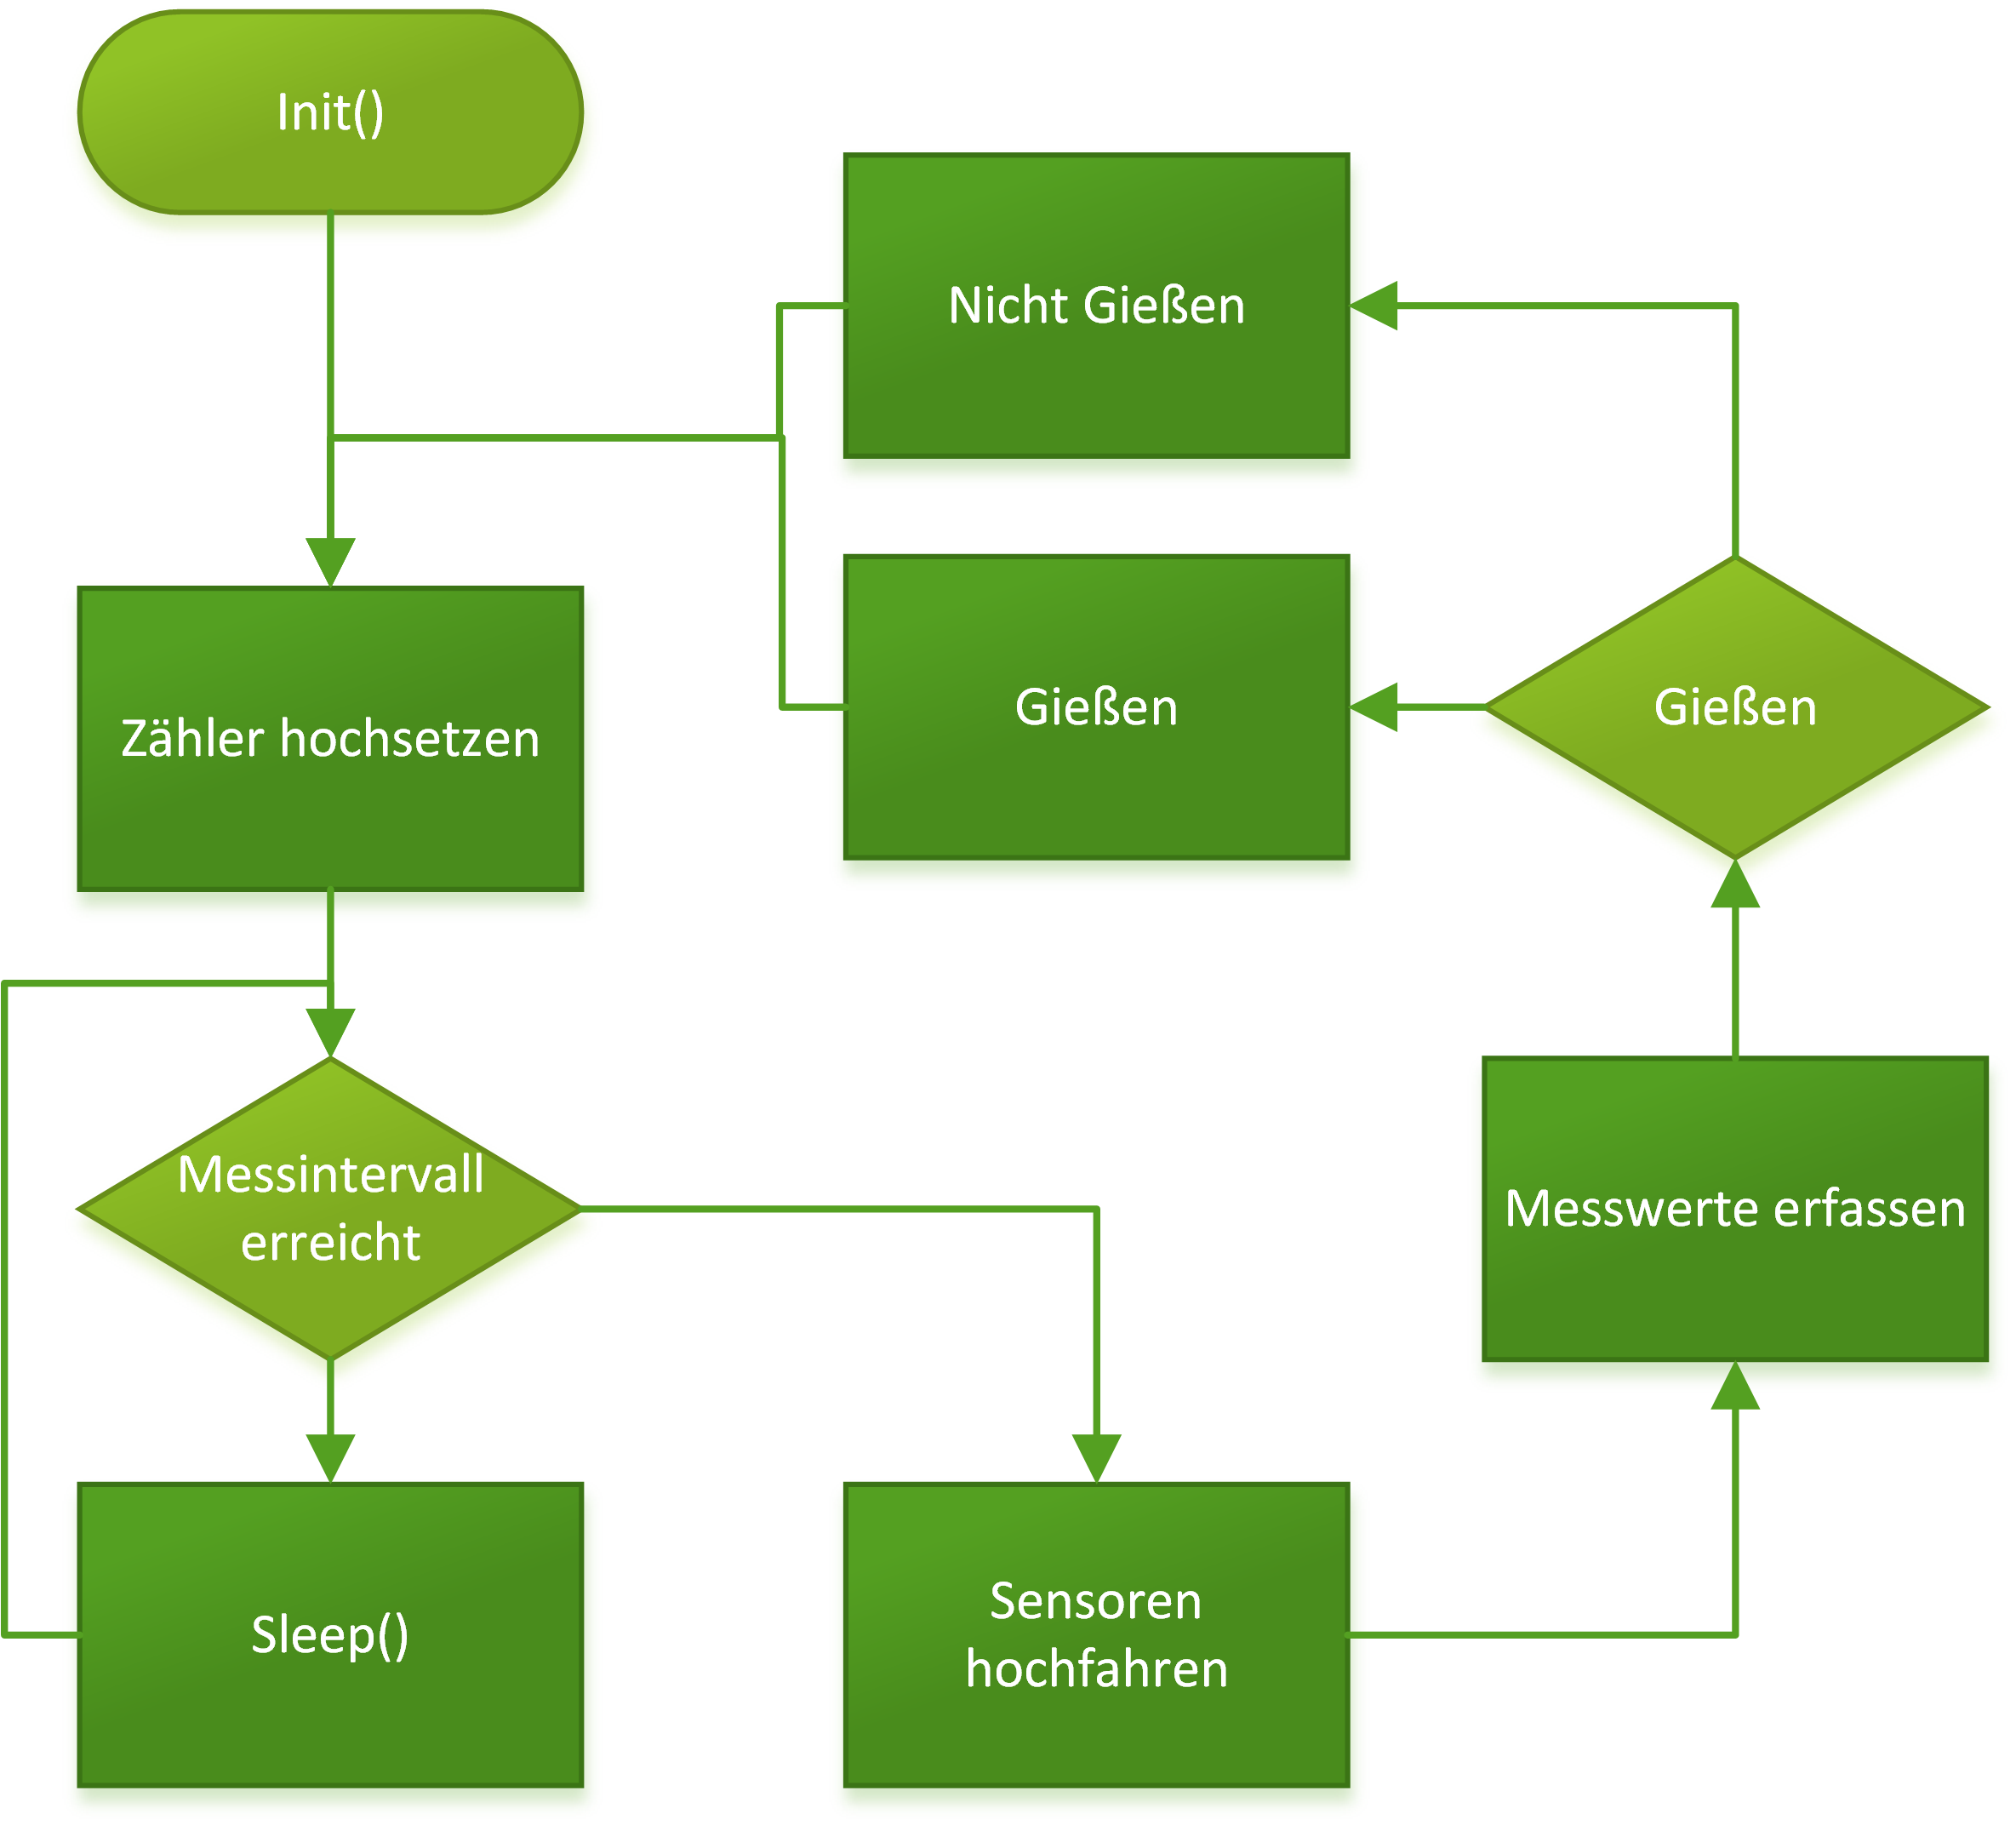
\includegraphics[width=0.8\linewidth]{Diagramme/SV_Ablaufdiagramm.png}
	\caption{Ablaufplan des Programms der Sparversion}
	\label{fig-SV_Ablaufplan}
\end{figure}

	Der Ablaufplan (Abbildung \ref{fig-SV_Ablaufplan}) der Sparversion wurde vereinfacht. Das Programm läuft linear immer wieder durch.
	Die meiste Zeit verbringt das System in der \glqq Sleep"~Schleife\grqq in dem nach jedem Timer"~Überlauf der Zähler um eins dekrementiert wird.
	Nach ungefähr 3 Stunden ist der Zähler klein genug und das Programm fährt die Sensoren hoch, indem er sie über den Transistor mit Strom versorgt.
	Dann erfolgt die Messung der Sensorwerte.
	Anhand der Sensorwerte wird nun entschieden ob gegossen wird.
	Nachdem Gießen wird der Zähler wieder hochgestellt und das Programm beginnt von vorne.
	\subsubsection{Kalbrierung der Sensoren}
	Da der Bodensensoren für jede Pflanze, jeden Boden und teilweise jede Einstich"-stelle im Boden neu kalibriert wird, wurde über diesen Prozess Gedanken gemacht.
	Es wurde entschieden dies manuell zu machen. 
	Dazu wird der Sensor in den trockenen Boden gesteckt und über die Vorschaltung mit Strom versorgt.
	Die Spannungsquelle an der Vorschaltung auf 5\,V gestellt und mit einem Multimeter die Spannung zwischen analog Ausgang und Grund gemessen.
	Nun wird solange gegossen bis die Erde feucht genug erscheint, die dazu passende Spannung wird notiert.
	Mit Hilfe der Formel \begin{math} { \frac{Messwert}{5,0\,V} } \times 1023 \end{math} wird der Wert errechnet, der in das Programm in die Definiton 
	\begin{verbatim}
	#define FEUCHTE	
	\end{verbatim} 
	eingetragen wird.
	
	
	
	\subsection{Kostenplan}

	\begin{table}[!h]
		\centering
		\onehalfspacing
		\footnotesize
		\caption{Kosten für eine  Sparversion Gießanlage}
		\label{Kosten für eine Sparversion Giesanlage}
	\begin{tabular}{|l|ll|}
			\hline
		\textit{Bauteil} & \textit{Kosten} & \textit{Bezugsquelle} \\
		\hline
		Arduino Nachbau & ca. 3 \euro & ebay \\
		Bodensensoren & ca. 2 \euro & ebay \\
		Zahnradpumpe & 2,95 \euro & Pollin \\
		Gehäuse	& 1,50 \euro & Pollin \\
		Hauptplatine & ca. 5,5 \euro & FabLAB \\
		\hline
		Gesamt: & ca 15 \euro & \\
		\hline
	\end{tabular}
	\end{table}
	
	  	
	Allein auf Grund des fehlenden XBee-Moduls halbiert sich der Preis der Anlage.
	Dazu kommt das fehlende Display, das kleinere Gehäuse und günstigere Hauptplatine.
	So ist der Nachbau der Sparversion ca. 15 \euro\ teuer. 
	In Tabelle \ref{Kosten für eine Sparversion Giesanlage} sind die Kosten nochmal zusammen getragen.
	 

	